\appendix
\renewcommand{\thesection}{APPENDIX \Alph{section}}

\section{} \label{appendix:A}

\subsection{Az állapotsűrűség nemrelativisztikus számítása}
Keressük a \ref{eq:8}. egyenletben leírt $dn \left( E, E_{\nu} \right)$ állapotszám egyváltozós alakját. Ezt a minden $E_{\nu}$-re történő kiintegrálással és egy $\left( E_{\nu} - E - Q \right)$ argumentumú Dirac-deltával kaphatjuk meg, ahol az utóbbi az energiamegmaradást érvényesítendő jelenik meg az egyenletben \citep{akos}. Az integrál alakja a következő ebben az esetben:

\begin{equation} \label{eq:19}
dn \left( E \right)
=
\int_{E_{\nu}} dn \left( E, E_{\nu} \right) * \delta \left( E_{\nu} - E - Q \right)
\end{equation}
\begin{equation} \label{eq:20}
dn \left( E \right)
=
C_{1} * \int_{E_{\nu}} \left( p_{e}^{2} \frac{dp_{e}}{dE} p_{\nu}^{2} \frac{dp_{\nu}}{dE_{\nu}} \right) * \delta \left( E_{\nu} - E - Q \right) dE dE_{\nu}
\end{equation}
Ahol $C_{1}$ egy soktagú konstans. Ennek az integrálnak az értéke a Dirac-delta azonosságai alapján egyből felírható:

\begin{equation} \label{eq:21}
dn \left( E \right)
=
C_{1} * \left. p_{e}^{2} \frac{dp_{e}}{dE} p_{\nu}^{2} \frac{dp_{\nu}}{dE_{\nu}} \right|_{E_{\nu} = Q - E} dE
\end{equation}
Melyből az állapotsűrűség $dE$-vel történő leosztás után kapható:

\begin{equation} \label{eq:22}
\frac{dn \left( E \right)}{dE}
=
C_{1} * \left. p_{e}^{2} \frac{dp_{e}}{dE} p_{\nu}^{2} \frac{dp_{\nu}}{dE_{\nu}} \right|_{E_{\nu} = Q - E}
\end{equation}
nemrelativisztikus esetben a \ref{eq:12}. és \ref{eq:13}. egyenletek helyettesítjük be az elektronra, valamint felhasználjuk a neutrínóra vonatkozó \ref{eq:10}. és \ref{eq:11}. képleteket is.

\begin{equation} \label{eq:23}
\frac{dn \left( E \right)}{dE}
=
C_{1} * \left( \sqrt{2 m_{e} E} \right)^{2} \frac{m_{e}}{\sqrt{2 m_{e} E}} * \left. \left( \frac{E_{\nu}}{c} \right)^{2} \right|_{E_{\nu} = Q - E} \frac{1}{c}
=
C_{1} * \frac{2 m_{e}^{2} E}{\sqrt{2 m_{e} E}} * \frac{\left( Q - E \right)^{2}}{c^{3}}
\end{equation}
A konstans értékeket (beleértve $C_{1}$-et is) egy $C_{2}$ konstansba összevonva a végleges állapotsűrűséget nemrelativisztikus esetben az alábbi függvény adja:

\begin{equation} \label{eq:24}
\boxed{
\frac{dn \left( E \right)}{dE}
=
C_{2} * \sqrt{E} \left( Q - E \right)^{2}
}
\end{equation}

\subsection{Az állapotsűrűség relativisztikus számítása}
Relativisztikus esetben a \ref{eq:21}. egyenletbe a neutrínóra vonatkozó egyenletek mellett az elektronra a \ref{eq:14}. és \ref{eq:15}. alakokat használjuk. Elvégezve a behelyettesítést a következőket kapjuk:

\begin{align} \label{eq:25}
\frac{dn \left( E \right)}{dE}
&=
C_{1} * \left( \frac{1}{c} \sqrt{\left( E + m_{e} c^2 \right)^2 - m_{e}^{2} c^{4}} \right)^{2}
*
\frac{1}{c} \frac{E + m_{e} c^2}{\sqrt{\left( E + m_{e} c^2 \right)^2 - m_{e}^{2} c^{4}}}
*
\left. \left( \frac{E_{\nu}}{c} \right)^{2} \right|_{E_{\nu} = Q - E} \frac{1}{c}
= \nonumber \\
&=
C_{1} * \frac{1}{c^{2}} \left( \left( E + m_{e} c^2 \right)^2 - m_{e}^{2} c^{4} \right)
*
\frac{1}{c} \frac{E + m_{e} c^2}{\sqrt{\left( E + m_{e} c^2 \right)^2 - m_{e}^{2} c^{4}}}
*
\frac{\left( Q - E \right)^{2}}{c^{3}}
= \nonumber \\
&=
C_{1} * \frac{1}{c^{6}}
*
\underbrace{\sqrt{\left( E + m_{e} c^{2} \right)^{2} - m_{e}^{2} c^{4}}}_{c p_{e}}
*
\underbrace{\left( E + m_{e} c^{2} \right)}_{E_{\text{tot}}}
*
\left( Q - E \right)^{2}
\end{align}
A konstans értékeket újból összevonva ($C_{1}$-el együtt) egy $C_{3}$ konstansba a végleges eredményre a következőt kapjuk:

\begin{equation} \label{eq:26}
\boxed{
\frac{dn \left( E \right)}{dE}
=
C_{3} * p_{e} * E_{tot} * \left( Q - E \right)^{2}
}
\end{equation}

\subsection{A nemrelativisztikus esetben illesztett görbe}
Mind a nemrelativisztikus, mind pedig a relativisztikus esetben az $n \left( E \right)$ állapotszám függvényét szükséges illeszteni az elméleti görbére. Ezt a $dn \left( E \right)$ integrálásából kaphatjuk meg. Nemrelativisztikus esetben a \ref{eq:24}. egyenletet felhasználva:

\begin{align} \label{eq:27}
n \left( E \right)
&=
\int dn \left( E \right)
=
C_{2} * \int \sqrt{E} * \left( Q - E \right)^{2} dE
= \nonumber \\
&=
C_{2} *
\left(
\int \sqrt{E} * Q^2 dE
-
\int \sqrt{E} * 2QE dE
+
\int \sqrt{E} * E^{2} dE
\right)
\end{align}
Az integrálokat elvégezve a következő alakot kapjuk:

\begin{equation} \label{eq:28}
\boxed{
n \left( E \right)
=
C_{2} *
\left(
\frac{2}{3} E^{3/2} Q^{2} - \frac{2}{5} E^{5/2} * 2Q + \frac{2}{7} E^{7/2}
\right)
}
\end{equation}
Az illesztéshez ez alapján az alábbi paraméteres görbét használtam:

\begin{equation} \label{eq:29}
\boxed{
f \left( E \right)
=
p_{1} + p_{2} * E^{3/2} - p_{3} * E^{5/2} + p_{4} * E^{7/2}
}
\end{equation}
A Fermi-függvénnyel kibővített esetben ez kissé változott:

\begin{equation} \label{eq:30}
\boxed{
f \left( E \right)
=
p_{1} + \left( p_{2} + p_{3} * E^{2/3} - p_{4} * E^{5/2} + p_{5} * E^{7/2} \right) * F \left( E \right)
}
\end{equation}


\subsection{A relativisztikus esetben illesztett görbe}
Relativisztikus esetben az állapotszám $n \left( E \right)$ függvénye jóval bonyolultabb képet öltött, mint a nemrelativisztikus esetben. Itt a \ref{eq:26}. egyenlet eredményét kell behelyettesítsük az integrandusba:

\begin{equation} \label{eq:31}
n \left( E \right)
=
\int dn \left( E \right)
=
C_{3} * \int p_{e} * E_{tot} * \left( Q - E \right)^{2} dE
\end{equation}
Mely a $p_{e}$ és $E_{tot}$ értékekkel behelyettesítve:

\begin{equation} \label{eq:32}
n \left( E \right)
=
C_{3} * \frac{1}{c} * \int
\sqrt{\left( E + m_{e} c^{2} \right)^{2} - m_{e}^{2} c^{4}}
*
\left( E + m_{e} c^{2} \right)
*
\left( Q - E \right)^{2} dE
\end{equation}
Kibontva a zárójeleket ezt az alakot több integrál összegére bonthatjuk, azonban az átláthatóság és a számolás egyszerűsége kedvéért, előbb rendezzük át a gyökös formában szereplő $p_{e}$ alakját:

\begin{equation} \label{eq:33}
\sqrt{\left( E + m_{e} c^{2} \right)^{2} - m_{e}^{2} c^{4}}
=
\sqrt{E^{2} + 2Em_{e}c^{2}}
=
\sqrt{E \left( E + 2m_{e}c^{2} \right)}
\end{equation}
Ezt felhasználva 6 integrál összegére bontjuk a \ref{eq:32}. egyenletben szereplő integrált:

\begin{equation} \label{eq:34}
I_{1}
=
\int \sqrt{E \left( E + 2m_{e}c^{2} \right)} * E * Q^{2}\,dE
=
Q^{2} * \int \sqrt{E^{3} \left( E + 2m_{e}c^{2} \right)}\,dE
\end{equation}
\begin{equation} \label{eq:35}
I_{2}
=
- \int \sqrt{E \left( E + 2m_{e}c^{2} \right)} * E * 2QE\,dE
=
- 2Q * \int \sqrt{E^{5} \left( E + 2m_{e}c^{2} \right)}\,dE
\end{equation}
\begin{equation} \label{eq:36}
I_{3}
=
\int \sqrt{E \left( E + 2m_{e}c^{2} \right)} * E * E^{2}\,dE
=
\int \sqrt{E^{7} \left( E + 2m_{e}c^{2} \right)}\,dE
\end{equation}
\begin{equation} \label{eq:37}
I_{4}
=
\int \sqrt{E \left( E + 2m_{e}c^{2} \right)} * m_{e} c^{2} * Q^{2}\,dE
=
m_{e} c^{2} * Q^{2} * \int \sqrt{E \left( E + 2m_{e}c^{2} \right)}\,dE
\end{equation}
\begin{equation} \label{eq:38}
I_{5}
=
- \int \sqrt{E \left( E + 2m_{e}c^{2} \right)} * m_{e} c^{2} * 2QE\,dE
=
- m_{e} c^{2} * 2Q * \int \sqrt{E^{3} \left( E + 2m_{e}c^{2} \right)}\,dE
\end{equation}
\begin{equation} \label{eq:39}
I_{6}
=
\int \sqrt{E \left( E + 2m_{e}c^{2} \right)} * m_{e} c^{2} * E^{2}\,dE
=
m_{e} c^{2} * \int \sqrt{E^{5} \left( E + 2m_{e}c^{2} \right)}\,dE
\end{equation}
Az $n \left( E \right)$ állapotszám értéke ekkor felírható ezek segítségével az alábbi módon:

\begin{equation} \label{eq:40}
n \left( E \right)
=
C_{3} * \frac{1}{c} * \sum_{k = 1}^{6} I_{k}
\end{equation}
Az $I_{k}$ függvények mindegyike hasonló alakú, megoldásuk egzakt alakra hozható:

\begin{equation} \label{eq:41}
\int \sqrt{x^{n} * \left( x + a \right)}
=
\frac{2x \sqrt{x^{n} * \left( x + a \right)} * {}_{2}F_{1} \left( -\frac{1}{2}; \frac{n}{2} + 1; \frac{n}{2} + 2; -\frac{x}{a} \right)}{\left( n + 2 \right) \sqrt{\frac{x + a}{a}}} + C
\end{equation}
Ahol ${}_{2}F_{1} \left( a; b; c; z \right)$ a hipergeometrikus függvény. Átírva az egyes integrálokat a következőket kapjuk:

\begin{equation} \label{eq:42}
I_{1}
=
Q^{2}
*
\frac{2 E \sqrt{E^{3} * \left( E + 2m_{e}c^{2} \right)} * {}_{2}F_{1} \left( -\frac{1}{2}; \frac{3}{2} + 1; \frac{3}{2} + 2; -\frac{E}{2m_{e}c^{2}} \right)}{\left( 3 + 2 \right) \sqrt{\frac{E + 2m_{e}c^{2}}{2m_{e}c^{2}}}} + C_{I_{1}}
\end{equation}
\begin{equation} \label{eq:43}
I_{2}
=
- 2Q
*
\frac{2 E \sqrt{E^{5} * \left( E + 2m_{e}c^{2} \right)} * {}_{2}F_{1} \left( -\frac{1}{2}; \frac{5}{2} + 1; \frac{5}{2} + 2; -\frac{E}{2m_{e}c^{2}} \right)}{\left( 5 + 2 \right) \sqrt{\frac{E + 2m_{e}c^{2}}{2m_{e}c^{2}}}} + C_{I_{2}}
\end{equation}
\begin{equation} \label{eq:44}
I_{3}
=
\frac{2 E \sqrt{E^{7} * \left( E + 2m_{e}c^{2} \right)} * {}_{2}F_{1} \left( -\frac{1}{2}; \frac{7}{2} + 1; \frac{7}{2} + 2; -\frac{E}{2m_{e}c^{2}} \right)}{\left( 7 + 2 \right) \sqrt{\frac{E + 2m_{e}c^{2}}{2m_{e}c^{2}}}} + C_{I_{3}}
\end{equation}
\begin{equation} \label{eq:45}
I_{4}
=
m_{e}c^{2} * Q^{2}
*
\frac{2 E \sqrt{E * \left( E + 2m_{e}c^{2} \right)} * {}_{2}F_{1} \left( -\frac{1}{2}; \frac{1}{2} + 1; \frac{1}{2} + 2; -\frac{E}{2m_{e}c^{2}} \right)}{\left( 1 + 2 \right) \sqrt{\frac{E + 2m_{e}c^{2}}{2m_{e}c^{2}}}} + C_{I_{4}}
\end{equation}
\begin{equation} \label{eq:46}
I_{5}
=
- m_{e}c^{2} * 2Q
*
\frac{2 E \sqrt{E^{3} * \left( E + 2m_{e}c^{2} \right)} * {}_{2}F_{1} \left( -\frac{1}{2}; \frac{3}{2} + 1; \frac{3}{2} + 2; -\frac{E}{2m_{e}c^{2}} \right)}{\left( 3 + 2 \right) \sqrt{\frac{E + 2m_{e}c^{2}}{2m_{e}c^{2}}}} + C_{I_{5}}
\end{equation}
\begin{equation} \label{eq:47}
I_{6}
=
m_{e}c^{2}
*
\frac{2 E \sqrt{E^{5} * \left( E + 2m_{e}c^{2} \right)} * {}_{2}F_{1} \left( -\frac{1}{2}; \frac{5}{2} + 1; \frac{5}{2} + 2; -\frac{E}{2m_{e}c^{2}} \right)}{\left( 5 + 2 \right) \sqrt{\frac{E + 2m_{e}c^{2}}{2m_{e}c^{2}}}} + C_{I_{6}}
\end{equation}
Jelöljünk minden hipergeometrikus függvényt az adott $I_{k}$-hoz tartozó $n$ értékkel. Így tehát

\begin{equation} \label{eq:48}
{}_{2}F_{1} \left( a; b; c; z \right)
\equiv
{}_{2}F_{1} \left( n \right)
\end{equation}
Nem elhagyva a konstans értékeket, egyszerűsítsük a fenti kifejezéseket:

\begin{multicols}{2}
\begin{equation} \label{eq:49}
I_{1}
=
Q^{2}
*
\frac{2 E^{5/2} * \sqrt{E + 2m_{e}c^{2}}}{5 \sqrt{\frac{E + 2m_{e}c^{2}}{2m_{e}c^{2}}}} * {}_2F_{1} \left( 3 \right)
\end{equation}
\begin{equation} \label{eq:50}
I_{2}
=
- 2Q
*
\frac{2 E^{7/2} * \sqrt{E + 2m_{e}c^{2}}}{7 \sqrt{\frac{E + 2m_{e}c^{2}}{2m_{e}c^{2}}}} * {}_2F_{1} \left( 5 \right)
\end{equation}
\begin{equation} \label{eq:51}
I_{3}
=
\frac{2 E^{9/2} * \sqrt{E + 2m_{e}c^{2}}}{9 \sqrt{\frac{E + 2m_{e}c^{2}}{2m_{e}c^{2}}}} * {}_2F_{1} \left( 7 \right)
\end{equation}
\begin{equation} \label{eq:52}
I_{4}
=
m_{e}c^{2} * Q^{2}
*
\frac{2 E^{3/2} * \sqrt{E + 2m_{e}c^{2}}}{3 \sqrt{\frac{E + 2m_{e}c^{2}}{2m_{e}c^{2}}}} * {}_2F_{1} \left( 1 \right)
\end{equation}
\begin{equation} \label{eq:53}
I_{5}
=
- m_{e}c^{2} * 2Q
*
\frac{2 E^{5/2} * \sqrt{E + 2m_{e}c^{2}}}{5 \sqrt{\frac{E + 2m_{e}c^{2}}{2m_{e}c^{2}}}} * {}_2F_{1} \left( 3 \right)
\end{equation}
\begin{equation} \label{eq:54}
I_{6}
=
m_{e}c^{2}
*
\frac{2 E^{7/2} * \sqrt{E + 2m_{e}c^{2}}}{7 \sqrt{\frac{E + 2m_{e}c^{2}}{2m_{e}c^{2}}}} * {}_2F_{1} \left( 5 \right)
\end{equation}
\end{multicols}
Az kifejezésekben szereplő törtek $\sqrt{E + 2m_{e}c^{2}}$-el egyszerűsíthetőek, valamint átrendezhetőek:

\begin{multicols}{2}
\begin{equation} \label{eq:55}
I_{1}
=
Q^{2}
*
\frac{2}{5} * E^{5/2} \sqrt{2m_{e}c^{2}} * {}_2F_{1} \left( 3 \right)
\end{equation}
\begin{equation} \label{eq:56}
I_{2}
=
- 2Q
*
\frac{2}{7} * E^{7/2} \sqrt{2m_{e}c^{2}} * {}_2F_{1} \left( 5 \right)
\end{equation}
\begin{equation} \label{eq:57}
I_{3}
=
\frac{2}{9} * E^{9/2} \sqrt{2m_{e}c^{2}} * {}_2F_{1} \left( 7 \right)
\end{equation}
\begin{equation} \label{eq:58}
I_{4}
=
m_{e}c^{2} * Q^{2}
*
\frac{2}{3} * E^{3/2} \sqrt{2m_{e}c^{2}} * {}_2F_{1} \left( 1 \right)
\end{equation}
\begin{equation} \label{eq:59}
I_{5}
=
- m_{e}c^{2} * 2Q
*
\frac{2}{5} * E^{5/2} \sqrt{2m_{e}c^{2}} * {}_2F_{1} \left( 3 \right)
\end{equation}
\begin{equation} \label{eq:60}
I_{6}
=
m_{e}c^{2}
*
\frac{2}{7} * E^{7/2} \sqrt{2m_{e}c^{2}} * {}_2F_{1} \left( 5 \right)
\end{equation}
\end{multicols}
Innentől kézzel átláthatatlan lenne tovább számolni, így a \texttt{Wolfram|Alpha} szoftverét hívtam segítségül, mely egyedi, szimbolikus számítási módjával viszonylag könnyen ki tudta hozni $n \left( E \right)$ végleges alakját. Az egyszerűség és átláthatóság kedvéért használjuk fel, hogy $m_{e}c^{2} \approx 511 keV$ és $Q = 156.5 keV$. Ekkor a végleges formula a következőképp fest:

\begin{align} \label{eq:61}
&n \left( E \right)
=
- C_{3} * \frac{1}{c}
*
\frac{1}{\sqrt{E (E + 1022)}} * 
\frac{1}{4} *
\left(
E \left( E + 1022 \right) * A \left( E \right) - \sqrt{E \left(E + 1022 \right)} * B \left( E \right)
\right)
\nonumber \\
&n \left( E \right)
=
- C_{3} * \frac{1}{c}
*
\frac{1}{4}
*
\frac{\sqrt{E \left(E + 1022 \right)}}{\sqrt{E (E + 1022)}} * 
\left(
\sqrt{E \left(E + 1022 \right)} * A \left( E \right) - B \left( E \right)
\right)
\nonumber \\
\to &\boxed{
n \left( E \right)
=
- C_{3} * \frac{1}{c}
*
\frac{1}{4}
* 
\left(
\sqrt{E \left(E + 1022 \right)} * A \left( E \right) - B \left( E \right)
\right) \quad \text{Mert $E > 0$}
}
\end{align}
Ahol $A \left( E \right)$ és $B \left( E \right)$ értéke:
\begin{equation} \label{eq:62}
A \left( E \right)
=
E^{3} + 643 E^{2} - 256778 * E + 6.67164*10^{7}
\end{equation}
\begin{equation} \label{eq:63}
B \left( E \right)
=
- 6.81842*10^{10} * \arcsinh \left(0.0312806 * \sqrt{E} \right)
\end{equation}
A nemrelativisztikus esethez hasonló módon a következő függvényt illesztettem relativisztikus esetben:

\begin{equation} \label{eq:64}
\boxed{
f \left( E \right)
=
p_{1} + p_{2} * \left( \sqrt{p_{3} + p_{4} * E^{2} + p_{5} * E} * A \left( E \right) - B \left( E \right) \right)
}
\end{equation}
Ahol most $A$ és $B$ a következő függvények voltak:

\begin{equation} \label{eq:65}
A \left( E \right)
=
p_{6} * E^{3} + p_{7} * E^{2} + p_{8} * E
\end{equation}
\begin{equation} \label{eq:66}
B \left( E \right)
=
p_{9} * \arcsinh \left(p_{10} * \sqrt{E} + p_{11} \right)
\end{equation}

A Fermi-függvényt is felhasználva a relativisztikus $f \left( E \right)$ függvény következő formát öltötte:

\begin{equation} \label{eq:67}
\boxed{
f \left( E \right)
=
p_{1} * F \left( E \right) + p_{2} * F \left( E \right) * \left( \sqrt{p_{3} + p_{4} * E^{2} + p_{5} * E} * A \left( E \right) - B \left( E \right) \right) + p_{+1}
}
\end{equation}

\subsection{A várható energia nemrelativisztikus számítása}

A számításhoz a \ref{eq:16}. egyenletben szereplő összefüggést használjuk, melybe a \ref{eq:24}. egyenletben kapott eredmény helyettesítjük be. Ilyenformán a következő alakot kapjuk:

\begin{equation} \label{eq:68}
\left< E \right>
=
\int_{0}^{Q} E P \left( E \right) dE
=
\int_{0}^{Q} E * \frac{dn \left( E \right) / dE}{\int_{0}^{Q} \left[ dn \left( E \right) / dE \right] dE} dE
\end{equation}
Előbb a $P \left( E \right)$ értékét számítjuk ki, mely a következő lesz:

\begin{equation} \label{eq:69}
P \left( E \right)
=
\frac{dn \left( E \right) / dE}{\int_{0}^{Q} \left[ dn \left( E \right) / dE \right] dE}
=
\frac{C_{2} * \sqrt{E} \left( Q - E \right)^{2}}{\int_{0}^{Q} \left[ C_{2} * \sqrt{E} \left( Q - E \right)^{2} \right] dE}
\end{equation}
A számlálóban és nevezőben megjelenő két konstans kiejti egymást. A végeredmény megadásához valójában csak a nevezőben szereplő integrál értékét kell kiszámítanunk:

\begin{align} \label{eq:70}
&\int_{0}^{Q} \sqrt{E} \left( Q - E \right)^{2} dE
=
\int_{0}^{Q} \sqrt{E} * \left( Q^{2} - 2QE + E^{2} \right) dE
= \nonumber \\
=&
\int_{0}^{Q} \sqrt{E} Q^{2} dE
-
\int_{0}^{Q} \sqrt{E} 2QE dE
+
\int_{0}^{Q} \sqrt{E} E^{2} dE
= \nonumber \\
=&
\left[ \frac{2}{3} * E^{3/2} Q^{2} \right]_{0}^{Q}
-
\left[ 2 * \frac{2}{5} * E^{5/2} * Q \right]_{0}^{Q}
+
\left[ \frac{2}{7} * E^{7/2} \right]_{0}^{Q}
= \nonumber \\
=&
\frac{2}{3} * Q^{3/2} Q^{2} - 2 * \frac{2}{5} * Q^{5/2} * Q + \frac{2}{7} * Q^{7/2}
=
\frac{2}{3} * Q^{7/2} - \frac{4}{5} * Q^{7/2} + \frac{2}{7} * Q^{7/2}
=
Q^{7/2} * \left( \frac{2}{3} - \frac{4}{5} + \frac{2}{7} \right)
\end{align}
Tehát végeredményben a nevezőben levő integrál értéke:

\begin{equation} \label{eq:71}
\int_{0}^{Q} \sqrt{E} \left( Q - E \right)^{2} dE
=
\frac{16}{105} Q^{7/2}
\end{equation}
Ebből a $P \left( E \right)$ értéke kiszámítható a \ref{eq:27}. egyenletbe behelyettesítve:

\begin{align} \label{eq:72}
P& \left( E \right)
=
\frac{\sqrt{E} \left( Q - E \right)^{2}}{\frac{16}{105} Q^{7/2}}
=
\frac{105}{16} \frac{\sqrt{E} Q^{2} - \sqrt{E} 2QE + \sqrt{E} E^{2}}{Q^{7/2}}
\nonumber \\
&P \left( E \right)
=
\frac{105}{16} \left( E^{1/2} Q^{-3/2} - E^{3/2} 2 Q^{-5/2} + E^{5/2} * Q^{-7/2} \right)
\end{align}
Ezen eredmény segítségével végre kiszámíthatjuk az energia várható értékének nagyságát:

\begin{align} \label{eq:73}
&\left< E \right>
=
\int_{0}^{Q} E * \frac{105}{16} \left( E^{1/2} Q^{-3/2} - E^{3/2} 2 Q^{-5/2} + E^{5/2} * Q^{-7/2} \right) dE
\nonumber \\
&\left< E \right>
=
\int_{0}^{Q} \frac{105}{16} \left( E^{3/2} Q^{-3/2} - E^{5/2} 2 Q^{-5/2} + E^{7/2} * Q^{-7/2} \right) dE
\nonumber \\
&\left< E \right>
=
\frac{105}{16}
*
\left(
Q^{-3/2} \int_{0}^{Q} E^{3/2} dE
-
2 Q^{-5/2} \int_{0}^{Q} E^{5/2} dE
+
Q^{-7/2} \int_{0}^{Q} E^{7/2} dE
\right)
\end{align}

Az itteni egyszerű integrálok során csak a felső integrálási határhoz tartozó értékek lesznek nem zérusak, így egyszerűen egy $E \to Q$ helyettesítéssel kapjuk meg a végleges eredményt az integrálok elvégzése után:
\begin{equation} \label{eq:74}
\left< E \right>
=
\frac{105}{16}
*
\left(
Q^{-3/2} \frac{2}{5} Q^{5/2} - 2Q^{-5/2} \frac{2}{7} Q^{7/2} + Q^{-7/2} \frac{2}{9} Q^{9/2}
\right)
=
\frac{105}{16}
*
\left(
\frac{2}{5} Q - \frac{4}{7} Q + \frac{2}{9} Q
\right)
\end{equation}
Így az $\left< E \right>$ végleges értéke nemrelativisztikus közelítésben:

\begin{equation} \label{eq:75}
\boxed{
\left< E \right>
=
\frac{105}{16}
*
\frac{16}{315}
*
Q
=
\frac{Q}{3}
}
\end{equation}

\newpage
\section{} \label{appendix:B}
\topskip0pt
\vspace*{\fill}
\begin{center}
    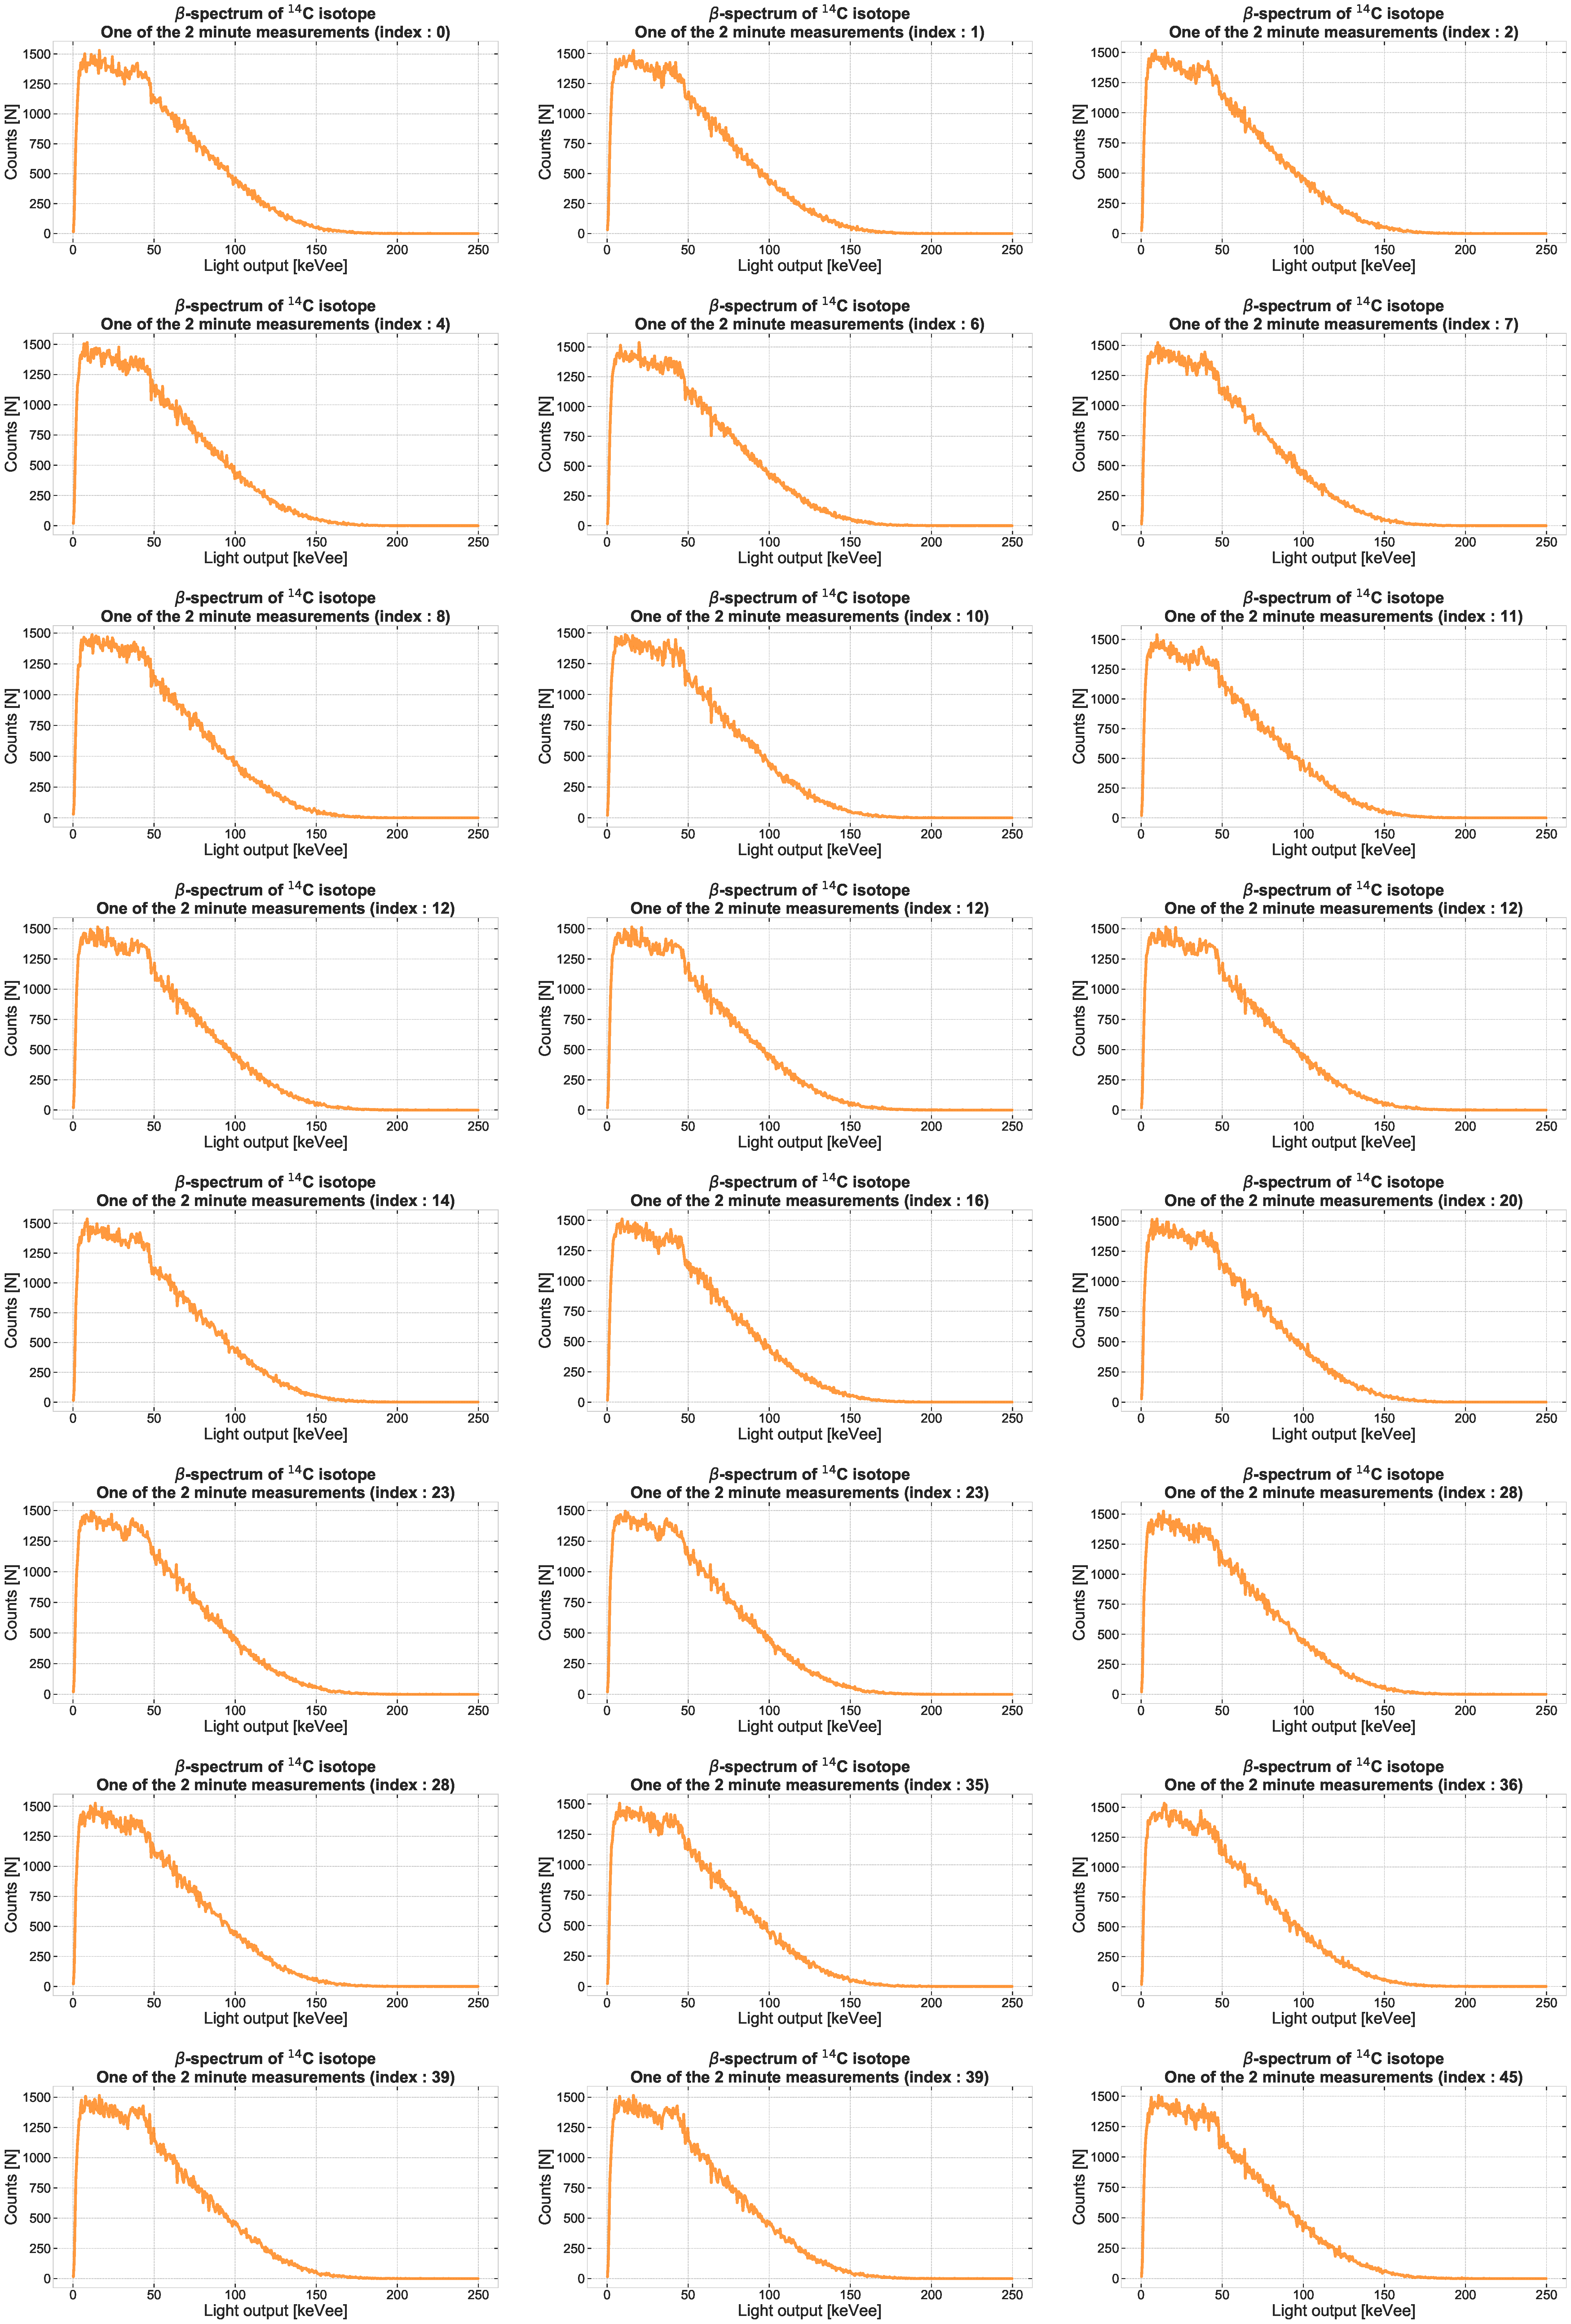
\includegraphics[width=\textwidth]{random_spectrums.pdf}
    \captionof{figure}{Az általunk vizsgált $^{14}$C különböző, egymás utáni 2 perces mérésekből származó $\beta$-spektrumai. Az összes 49 sikeres mérés közül 24 darab van az ábrára véletlenszerűen kiválasztva.} \label{fig:1}
\end{center}
\vspace*{\fill}
\newpage
\topskip0pt
\vspace*{\fill}
\begin{center}
    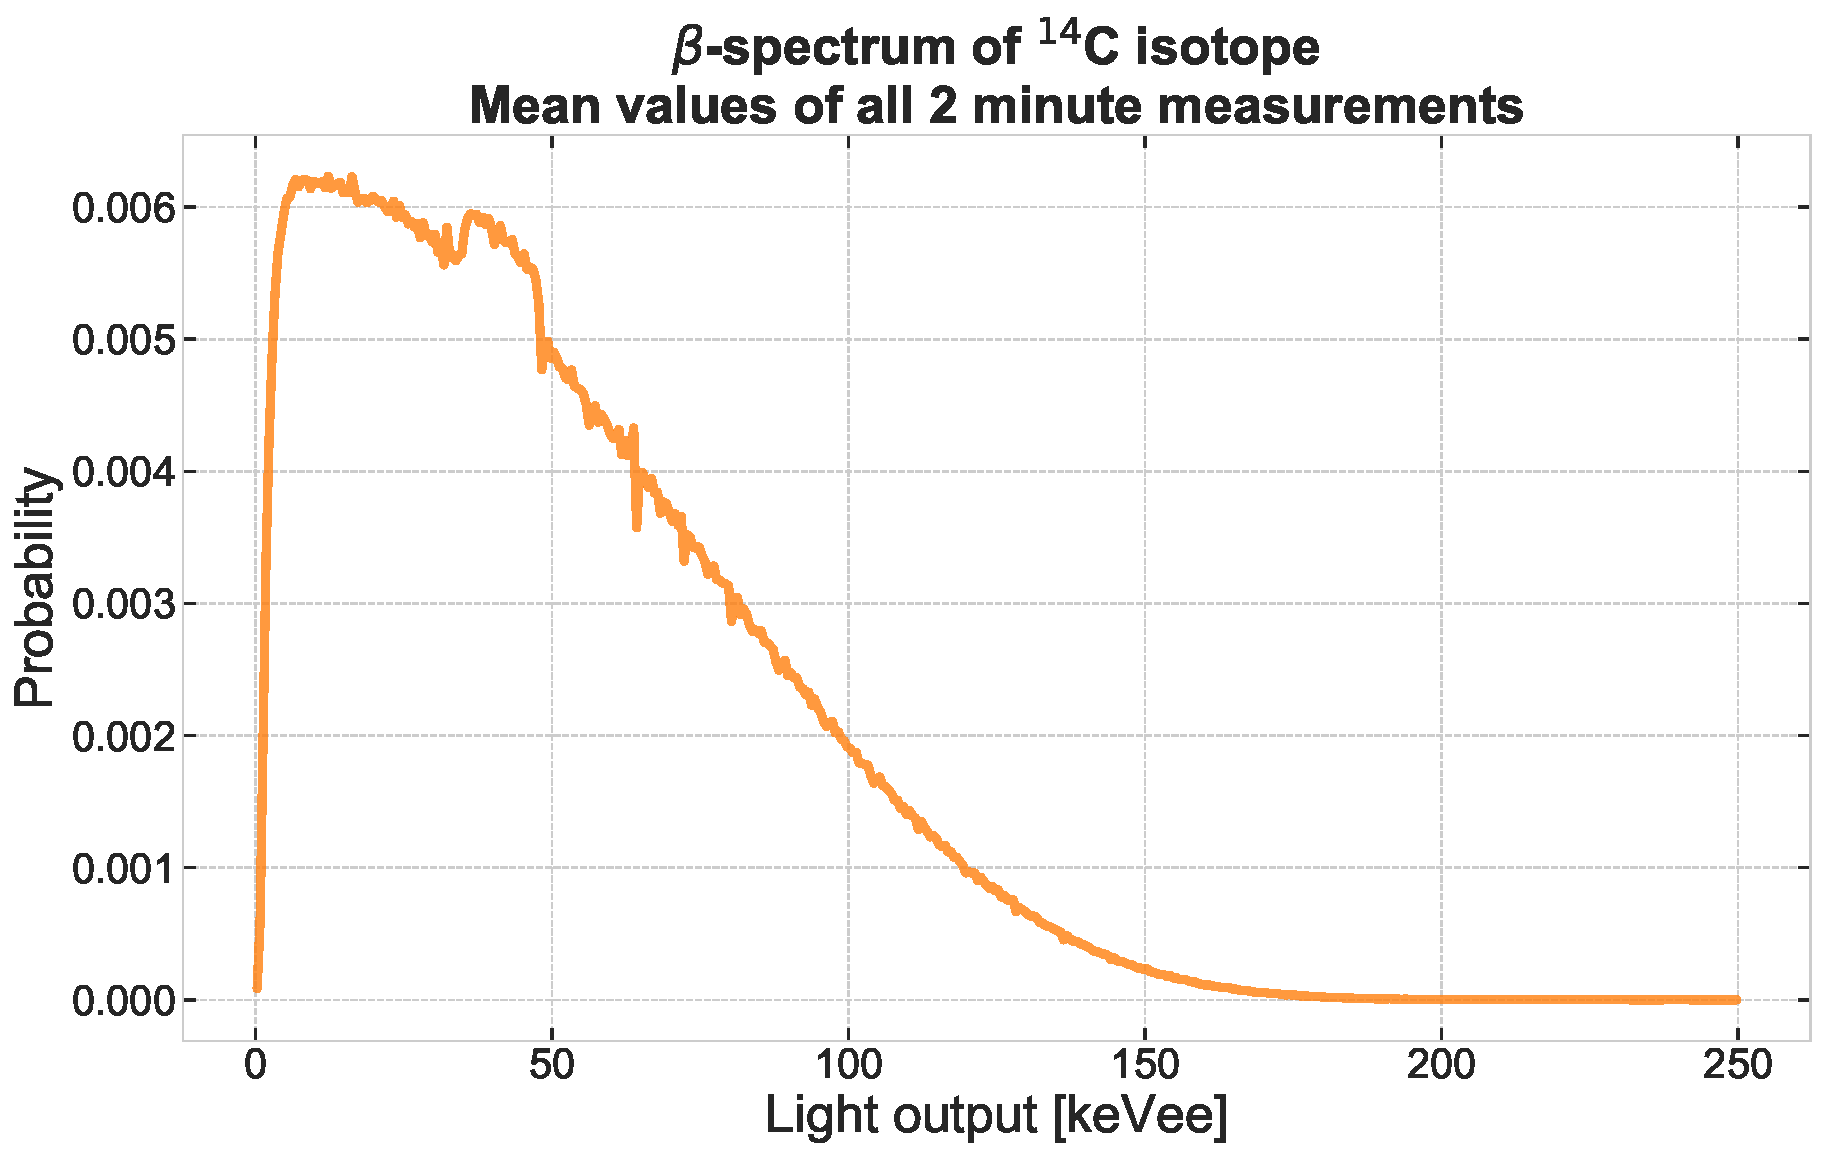
\includegraphics[width=\textwidth]{mean_spectrum.pdf}
    \captionof{figure}{Az általunk vizsgált $^{14}$C különböző, egymás utáni 2 perces mérésekből származó $\beta$-spektrumainak átlagolt értéke.} \label{fig:2}
\end{center}
\begin{center}
    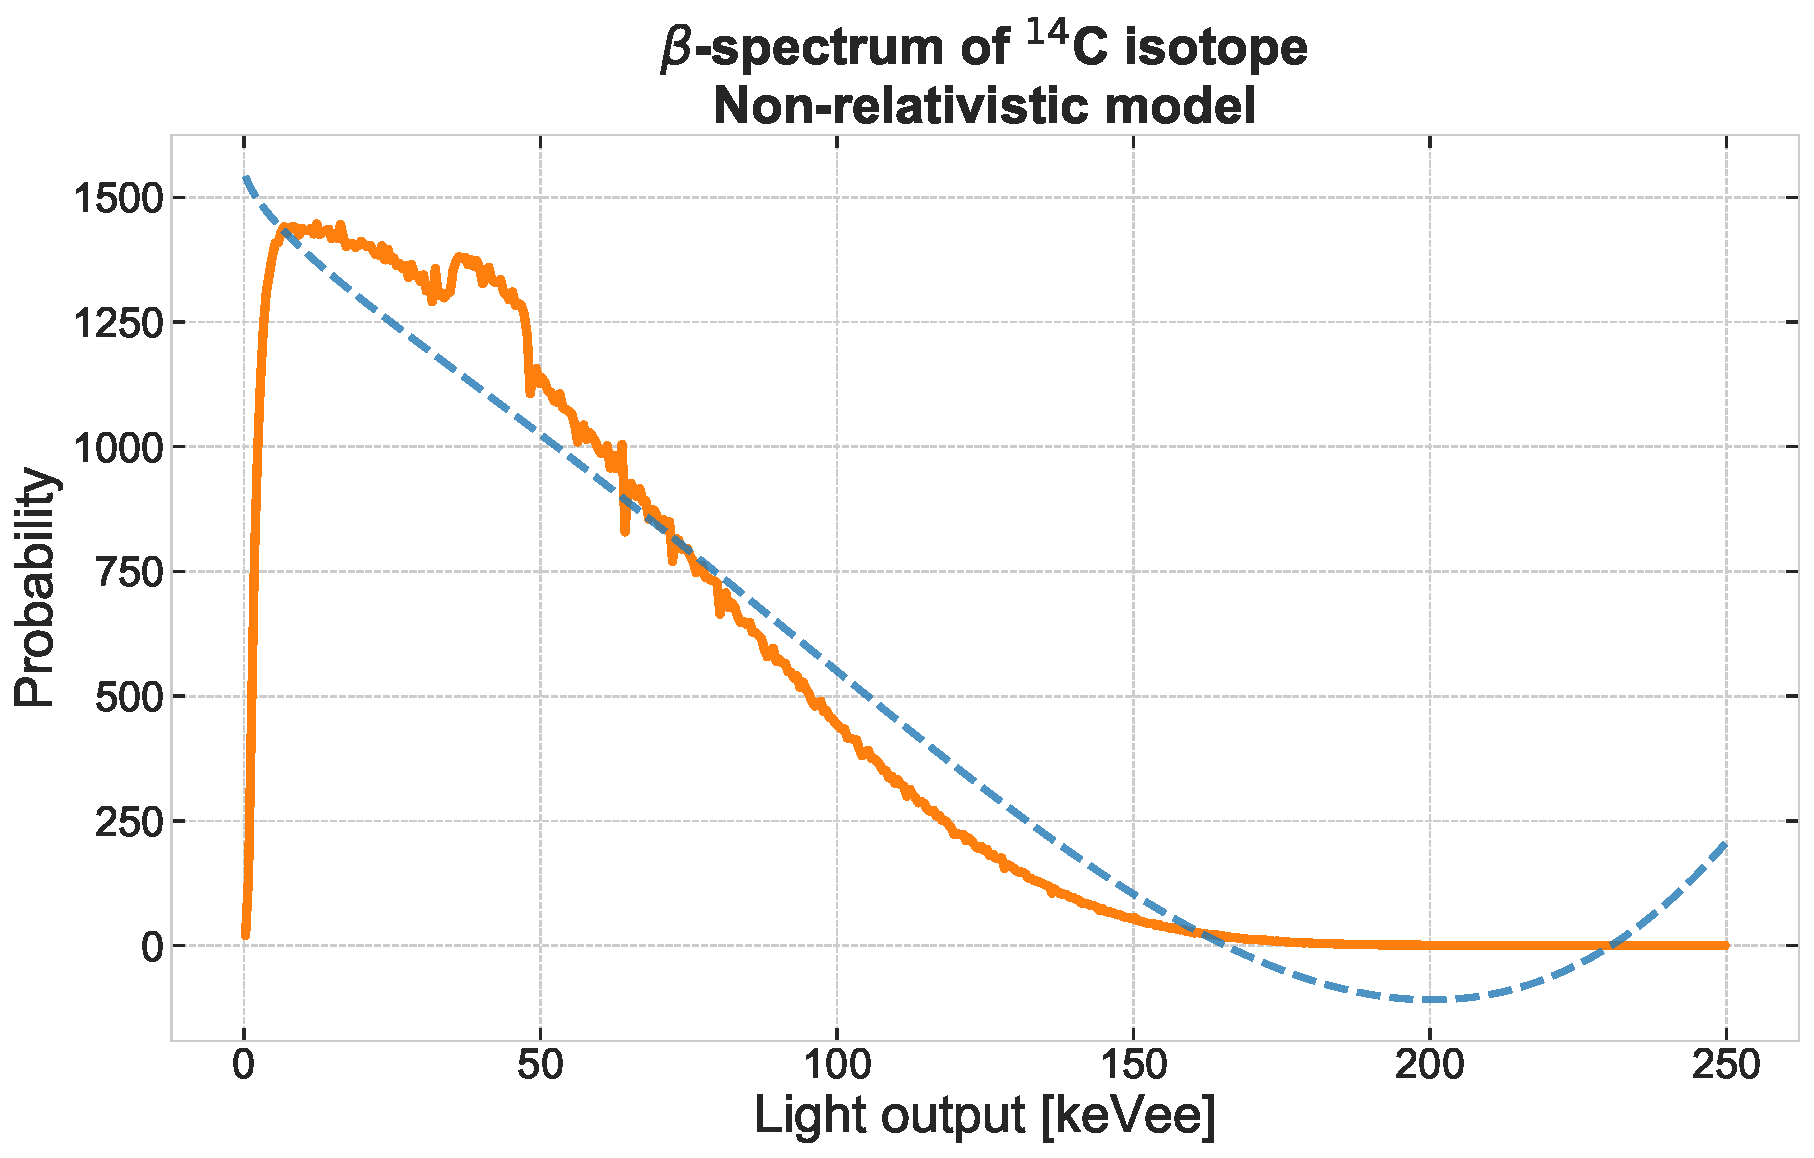
\includegraphics[width=\textwidth]{non_relat_fit.pdf}
    \captionof{figure}{Az általunk vizsgált $^{14}$C kiátlagolt spektrumára illesztett nemrelativisztikus függvény, mely egy túl jó közelítésben, de láthatóan visszaadja a $\beta$-spektrum kezdetben lecsengő alakját. Zérushelye a $^{14}$C karakterisztikus $156.5$ keV-es $Q$ értéke körül van.} \label{fig:3}
\end{center}
\vspace*{\fill}
\newpage
\topskip0pt
\vspace*{\fill}
\begin{center}
    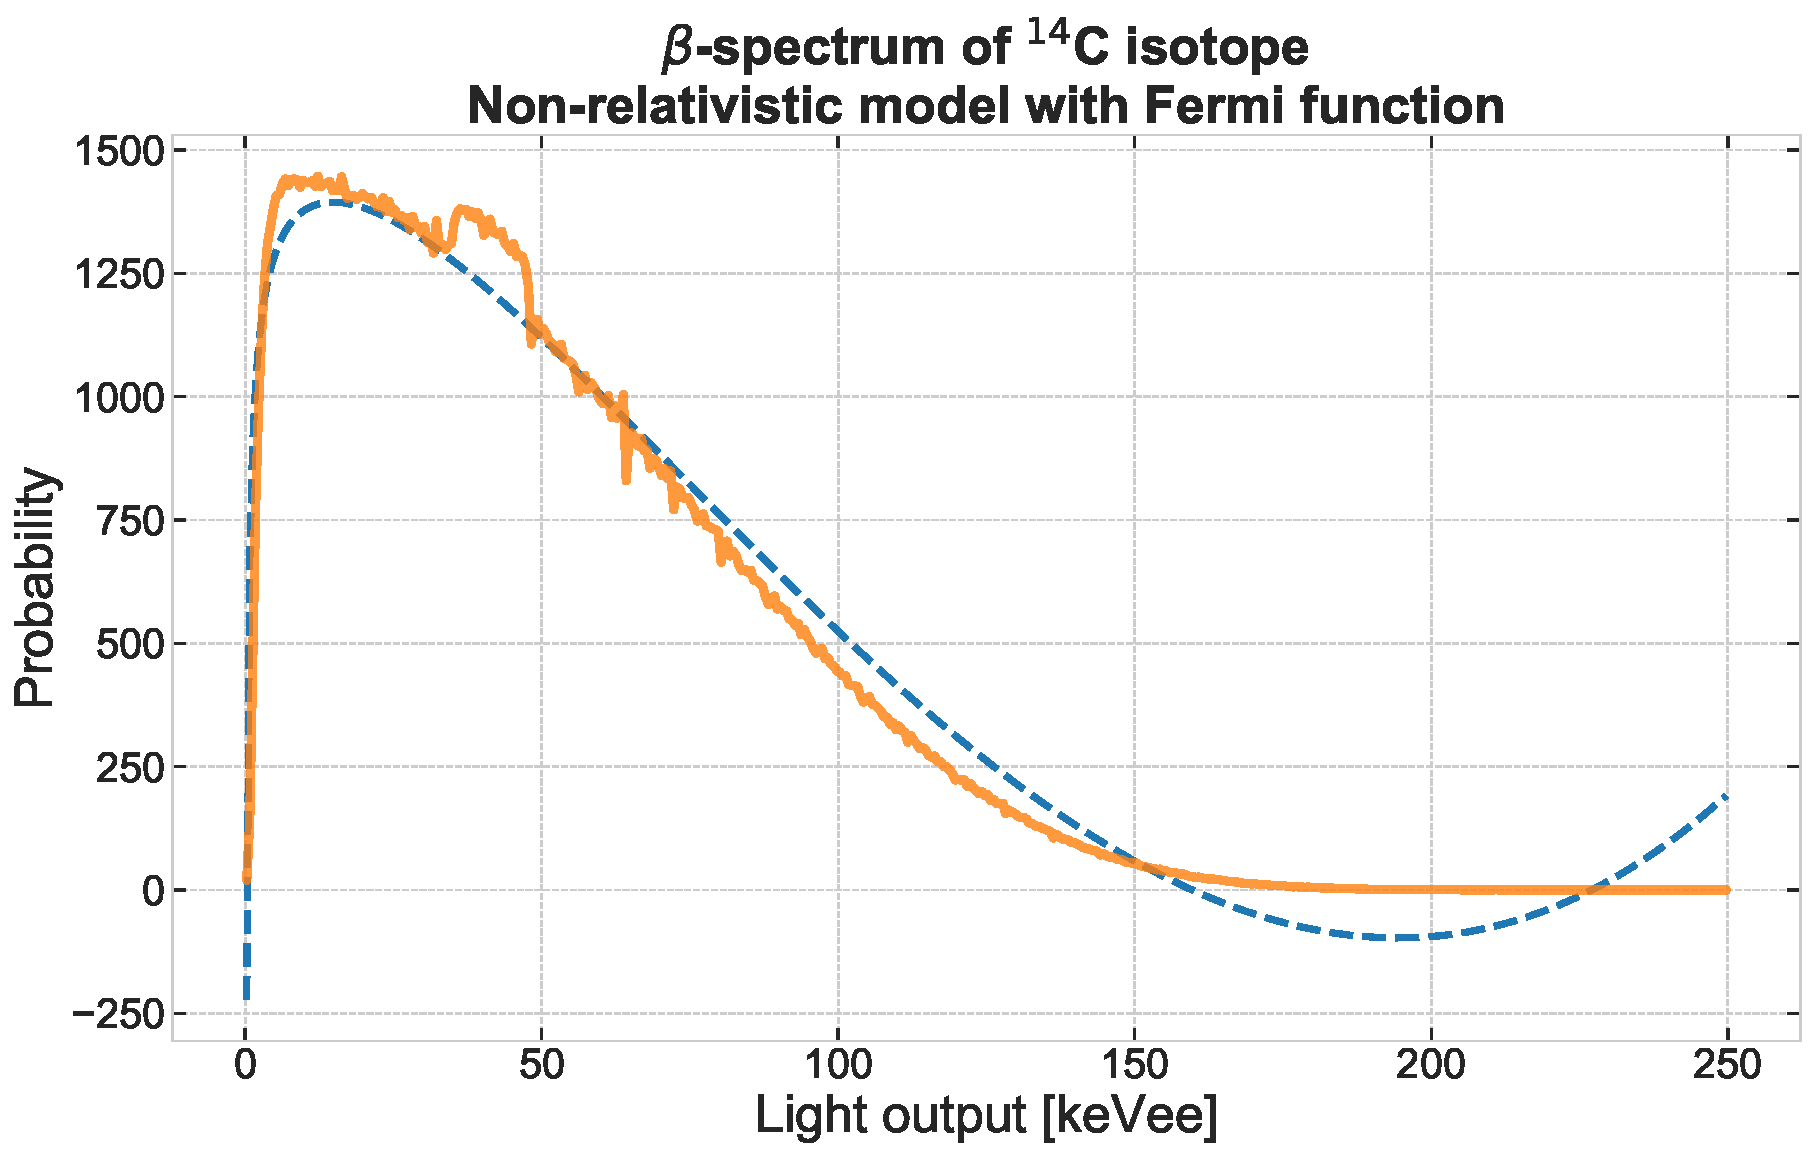
\includegraphics[width=\textwidth]{non_relat_fermi_fit.pdf}
    \captionof{figure}{Az általunk vizsgált $^{14}$C kiátlagolt spektrumára illesztett nemrelativisztikus függvény, mely a Fermi-függvény által nyújtott korrekciót felhasználva, az előzőnél sokkal jobban megközelíti a $\beta$-spektrum görbéjét. A zérushely itt is a $^{14}$C karakterisztikus $156.5$ keV-es $Q$ érték körül van.} \label{fig:4}
\end{center}
\begin{center}
    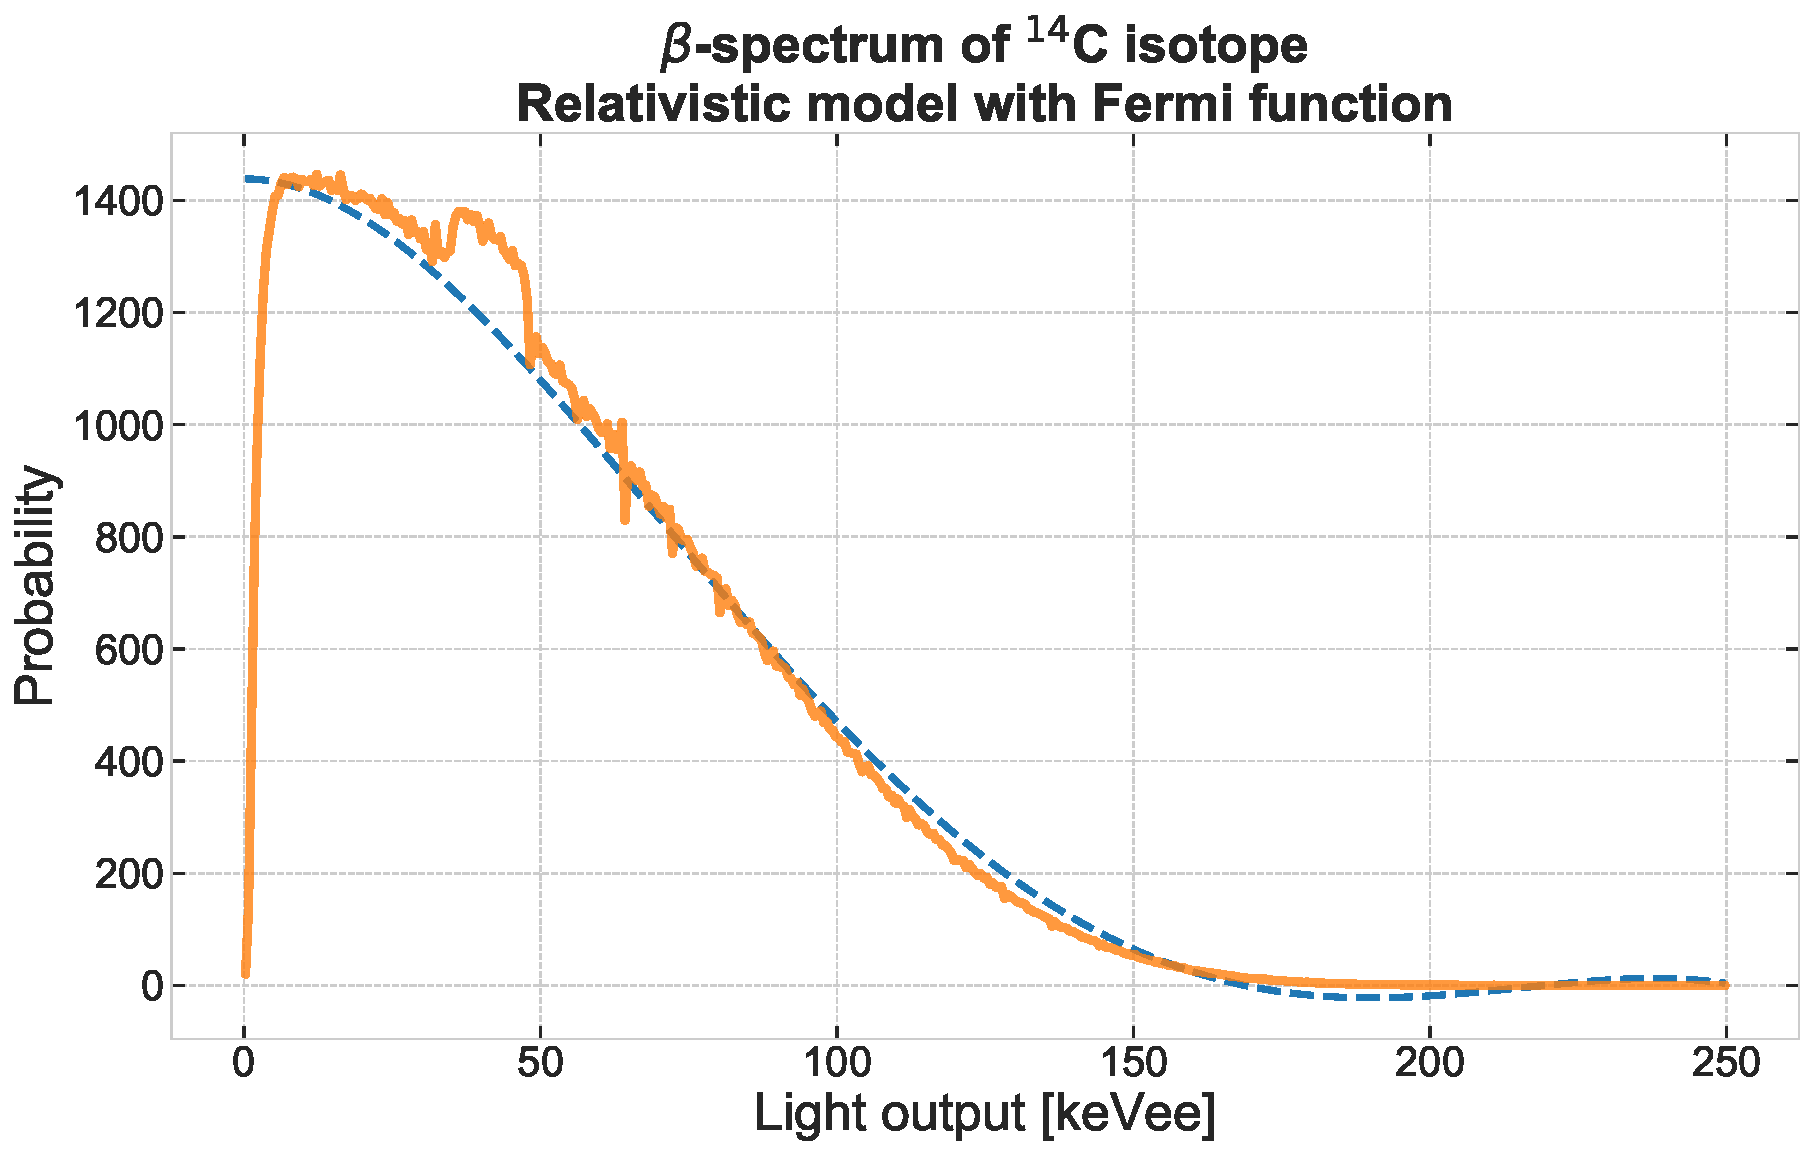
\includegraphics[width=\textwidth]{relat_fermi_fit.pdf}
    \captionof{figure}{Az általunk vizsgált $^{14}$C kiátlagolt spektrumára illesztett relativisztikus függvény, melyet a Fermi-függvénnyel korrigáltam. Zérushelye szintén a $^{14}$C karakterisztikus $156.5$ keV-es $Q$ értéke körül van és az előzőekkel ellentétben a nagyobb energiáknál már nem látszik felfutó él. Ennek az illesztett egyenletét \texttt{Wolfram|Alpha}-val számítottam ki egyenesen a \ref{eq:32}. egyenletből. A jegyzőkönyvben ennek értéke nem szerepel, mivel külsőre erősen felvállalhatatlan. Az illesztéshez használt programkód azonban megtalálható a GitHubomon, melynek linkje a hivatkozások között érhető el.} \label{fig:5}
\end{center}
\vspace*{\fill}
\newpage
\topskip0pt
\vspace*{\fill}
\begin{center}
    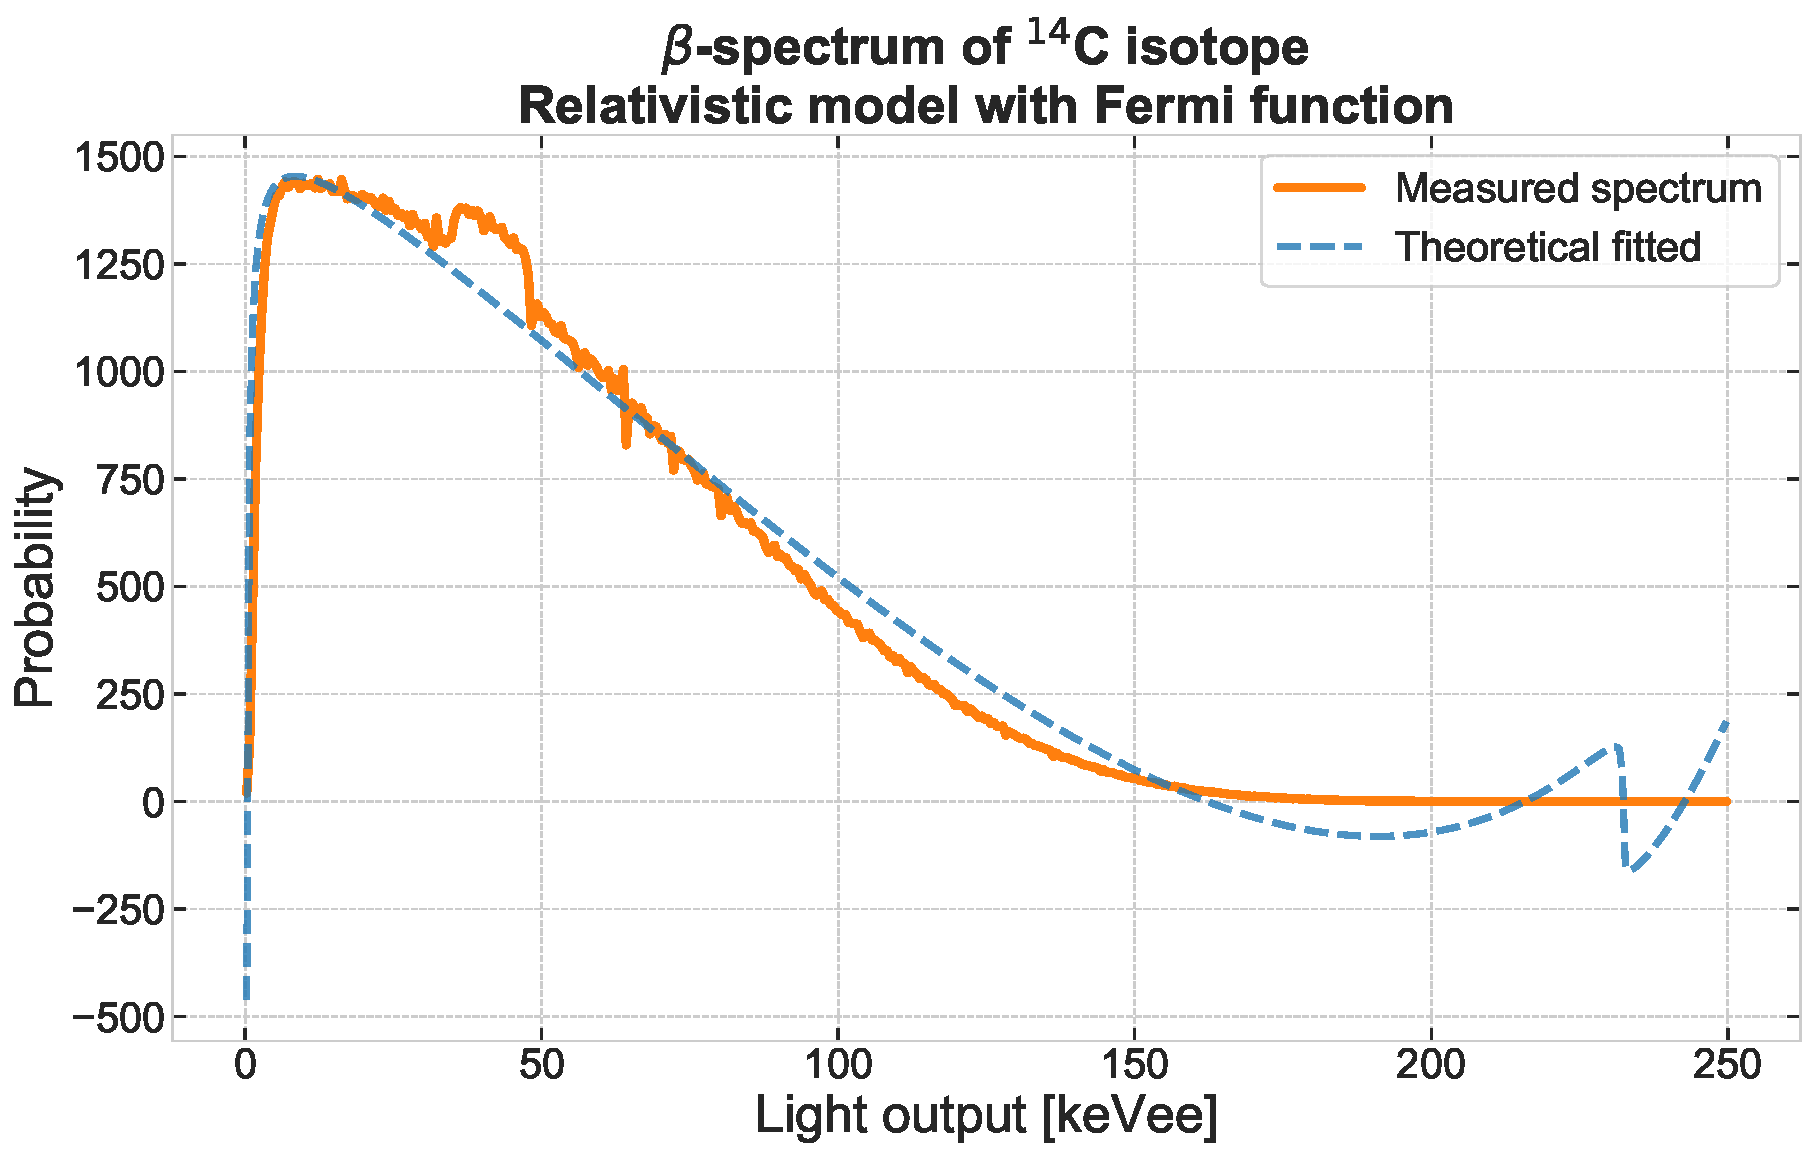
\includegraphics[width=\textwidth]{relat_fermi_fit2.pdf}
    \captionof{figure}{Az általunk vizsgált $^{14}$C kiátlagolt spektrumára illesztett relativisztikus függvény, melyet a Fermi-függvénnyel korrigáltam. Ennek értékét számítottam ki az \hyperref[appendix:A]{A.} függelékben. Míg a függvény elejét sokkal megfelelőbben leírja, mint a \ref{fig:5}. ábrán látható verzió, addig ennek a $Q$-érték körül már súlyos gondjai vannak. Emellett erősen hasonlít a függvénymenet a nemrelativisztikus esethez.} \label{fig:6}
\end{center}
\begin{center}
    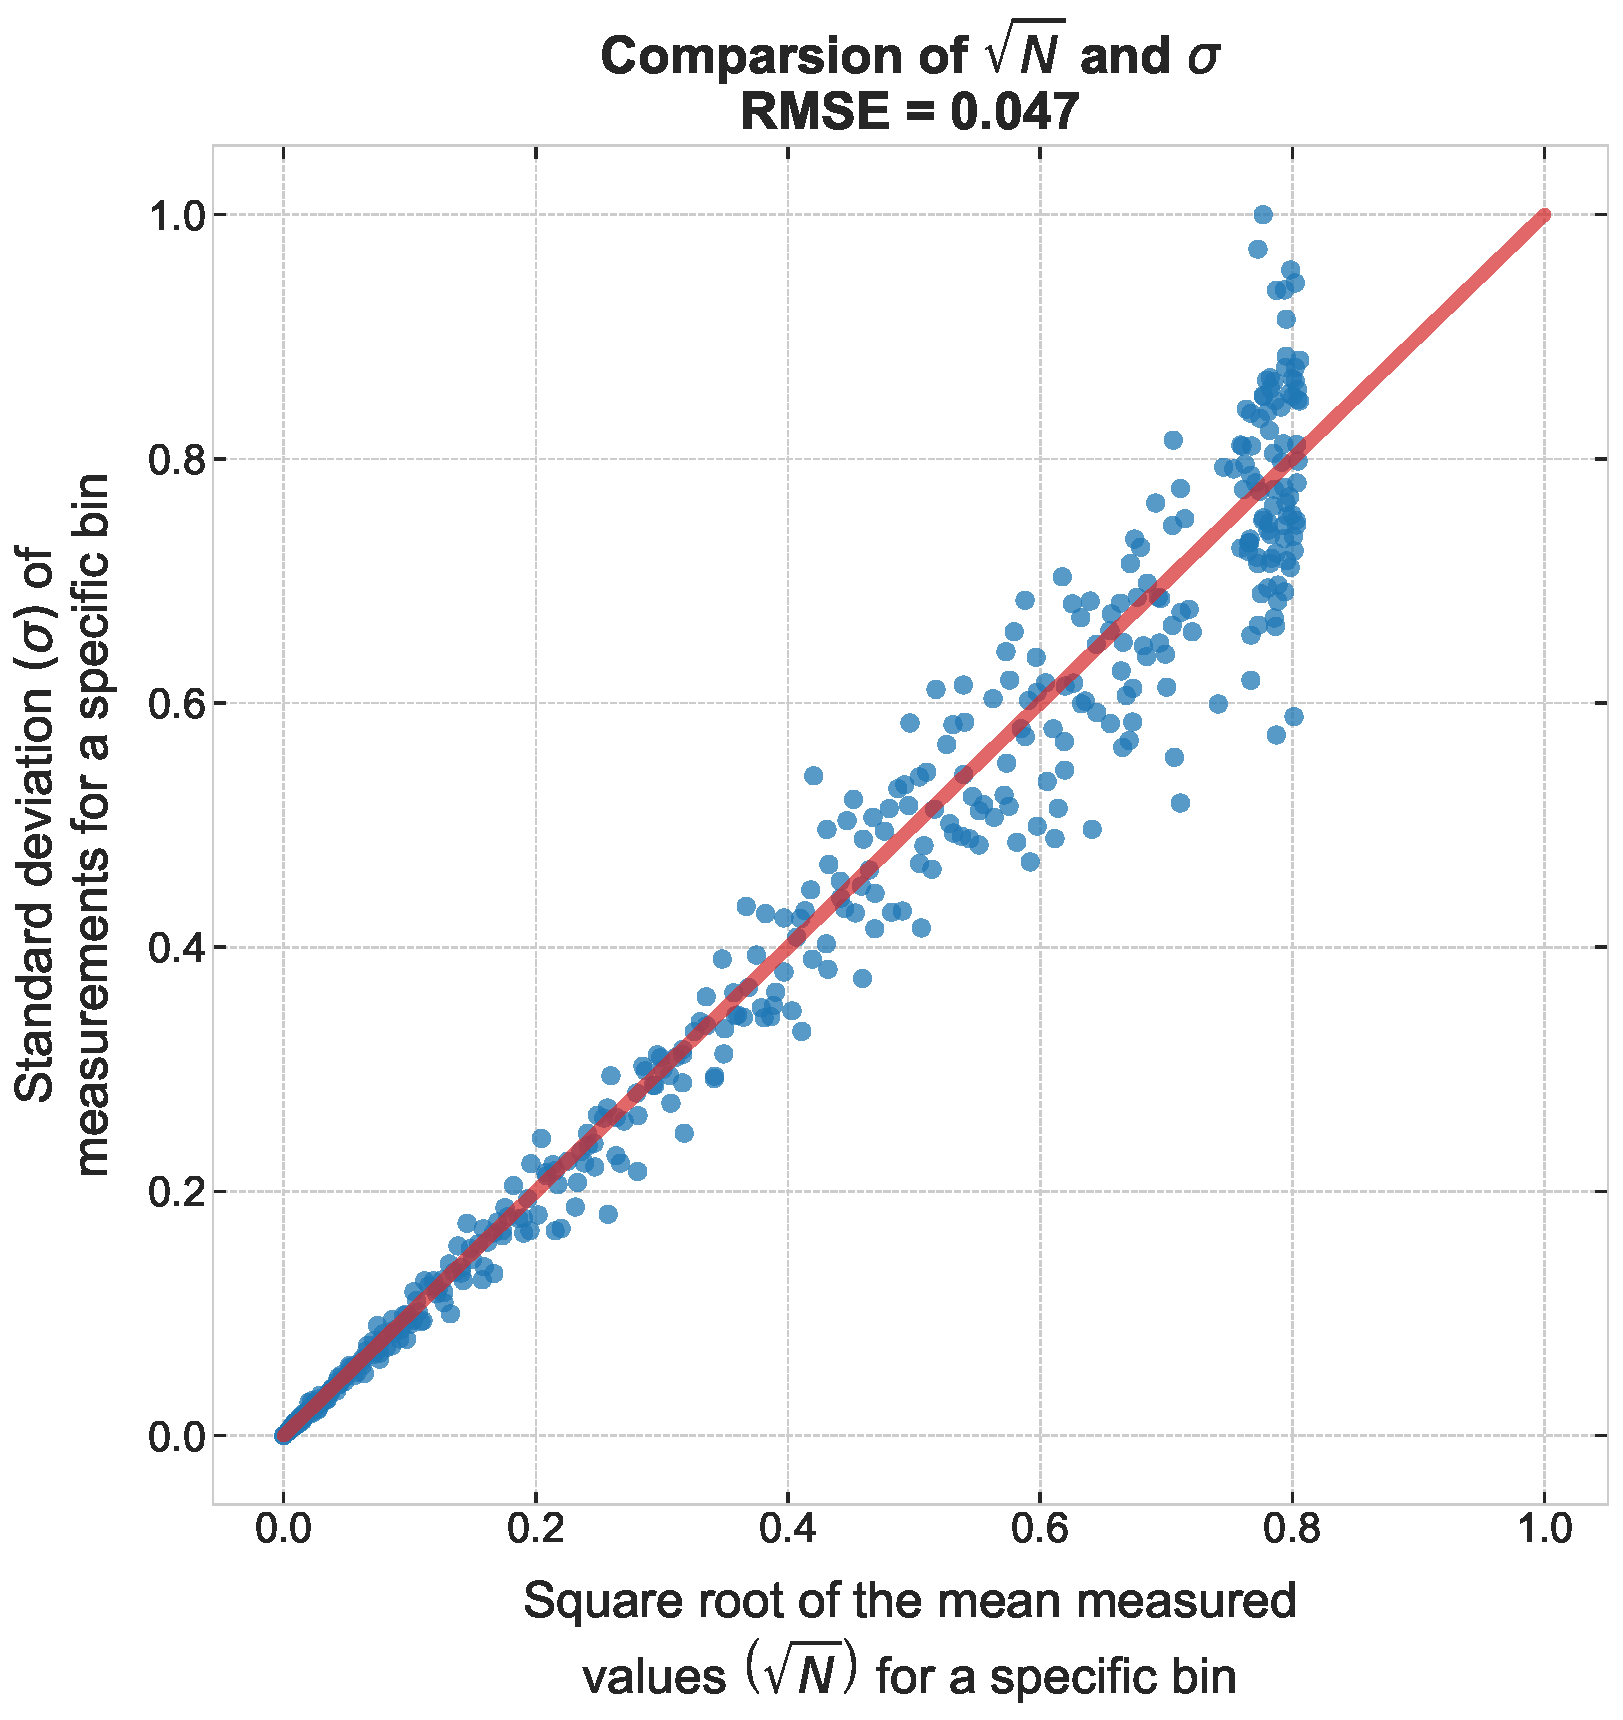
\includegraphics[width=0.8\textwidth]{error_compare.pdf}
    \captionof{figure}{Az egyes $N \left( E \right)$ értékek hibáját (szórását) közelíthetjük az $\sqrt{N}$ formulával. Ideális esetben a $\sqrt{N}$ -- $\sigma$ függvény a $45^{\circ}$-os egyenesre illeszkedik. Az ábrán ezen függvény ábrázoltam a meghatározott $\sqrt{N}$ és $\sigma$ értékek segítségével. Az illeszkedés hibáját a machine learning modelleknél bevett átlag négyzetes hiba gyökének kiszámításával vizsgáltam, mely értéke szintén az ábrán látható.} \label{fig:7}
\end{center}
\vspace*{\fill}